\documentclass{article}

\usepackage{graphicx}
\usepackage{amsmath}
\usepackage{hyperref}
\usepackage{comment} % Include the comment package
\usepackage{caption}
\usepackage{float} % for the H specifier
\usepackage{subcaption}
\usepackage{amsfonts}
\usepackage{amssymb}
\usepackage{graphicx}

\usepackage[a4paper, margin=1in]{geometry}
\usepackage{hyperref} % Load the hyperref package





\title{From Autoencoders to GANs, and Diffusion Models in Machine Learning}
\author{Filip Fabris \\ \href{mailto:filip.fabris@mail.polimi.it}{filip.fabris@mail.polimi.it}}
\date{\today}

\begin{document}

\begin{titlepage} % Start of the title page environment
\newcommand{\HRule}{\rule{\linewidth}{0.5mm}} % Defines a new command for horizontal lines, change thickness here

\center % Center everything on the page

%----------------------------------------------------------------------------------------
%	HEADING SECTIONS
%----------------------------------------------------------------------------------------
\textsc{\LARGE Politecnico di Milano}\\[1.5cm] % Name of your university/college
\textsc{\Large Project Report}\\[0.5cm] % Major heading such as course name
\textsc{\large 055697 - NUMERICAL ANALYSIS FOR MACHINE LEARNING}\\[0.5cm] % Minor heading such as course title

%----------------------------------------------------------------------------------------
%	TITLE SECTION
%----------------------------------------------------------------------------------------
\HRule \\[0.4cm]
{ \huge \bfseries From Autoencoders to GANs, and Diffusion Models in Machine Learning}\\[0.4cm] % Title of your document
\HRule \\[1.5cm]
 
%----------------------------------------------------------------------------------------
%	AUTHOR SECTION
%----------------------------------------------------------------------------------------
\begin{minipage}{0.4\textwidth}
\begin{flushleft} \large
\emph{Author:}\\
Filip Fabris % Your name
\\ \href{mailto:filip.fabris@mail.polimi.it}{filip.fabris@mail.polimi.it} % Your email
\end{flushleft}
\end{minipage}
~
\begin{minipage}{0.4\textwidth}
\begin{flushright} \large
\emph{Supervisor:} \\
Dr. Edie Miglio % Supervisor's Name
\\ \href{mailto:edie.miglio@polimi.it}{filip.fabris@mail.polimi.it} % Your email
\end{flushright}
\end{minipage}\\[2cm]

%----------------------------------------------------------------------------------------
%	DATE SECTION
%----------------------------------------------------------------------------------------
{\large \today}\\[2cm] % Date, change the \today to a set date if you want to be precise

%----------------------------------------------------------------------------------------
%	LOGO SECTION
%----------------------------------------------------------------------------------------
%\includegraphics{Logo}\\[1cm] % Include a department/university logo - this will require the graphicx package


\vfill % Fill the rest of the page with whitespace
\end{titlepage}
			
	\section{Introduction}
			
	Today deep learning is one of most active research fields in domain of machine learning. In this project we will examine three main concepts: Autoencoders, generative adversarial networks (GANs) and diffusion models. Goal of this project is to understand the mechanisms behind each concept, clarify their core principles and finally unravel the interconnections that exists between them. 
	To achieve this goal, we will first explain what Autoencoders are, then we will explain how GAN was invented from Autoencoders, and finally we will explain the rise of Defussion models
	
	\section{Autoencoders}

	Firstly lets just briefly explain what Autoencoders are.
	Autoencoders are a class of neural networks that are used in unsupervised learning tasks to learn compressed and meaningful representations of input data.
	They are designed to learn compressed and meaningful representations of input data.

	\begin{figure}[h]
		\centering
		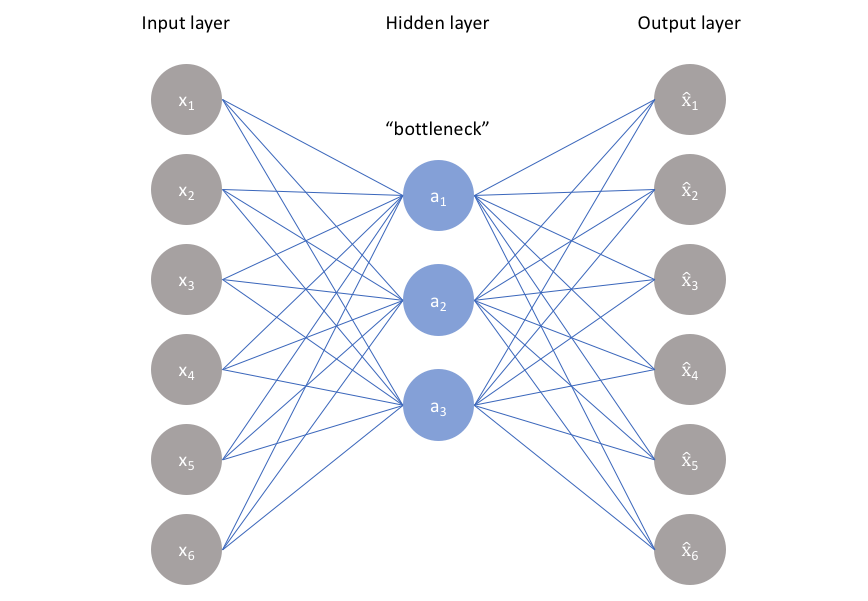
\includegraphics[width=0.5\linewidth]{images/bottleneck.png}
		\caption{Autoencoder architecture with a bottleneck component}
		\label{fig:bottleneck}
	\end{figure}

	Traditionally, autoencoders were used for dimensionality reduction, where the high-dimensional data can be represented in the low dimensional space, something like PCA. But the main difference is that PCAs were limited by their linearity and they couldn`t represent data with a high-dimensional non-linear manifold into a low dimensional space.
	
	Autoencoders can do that thanks to neural networks. This is why the autoencoder and its variants are used in a lot of applications which we will introduce in following sections.

		\subsection{For what are Autoencoders used?}
			Autoencoders find diverse applications in various domains. In this section, we explore some prominent use cases.

		\subsubsection{Dimensionality Reduction}

			The reconstructed image is the same as our input but with reduced dimensions. It helps in providing the similar image with a reduced pixel value.

			\begin{figure}[H]
				\centering
				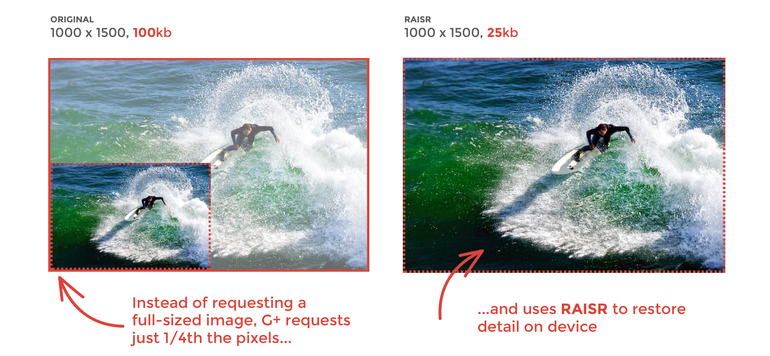
\includegraphics[width=0.8\linewidth]{images/dimensionality-reduction.png}
				\caption{Dimensionality reduction using autoencoders}
				\label{fig:dimensionality-reduction}
			\end{figure}

		\subsubsection{Data Denoising}

			Another application of auto encoders is data denoising.

			\begin{figure}[H]
				\centering
				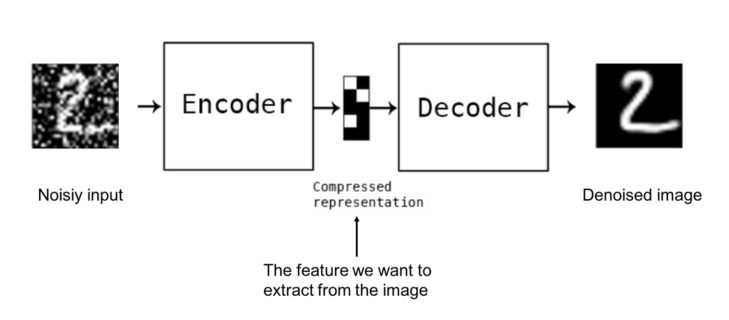
\includegraphics[width=0.8\linewidth]{images/denosing.png}
				\caption{Data denoising using autoencoders}
				\label{fig:denosing}
			\end{figure}

		\subsubsection{Feature variation}

			It extracts only the required features of an image and generates the output by removing any noise or unnecessary interruption.

			\begin{figure}[H]
				\centering
				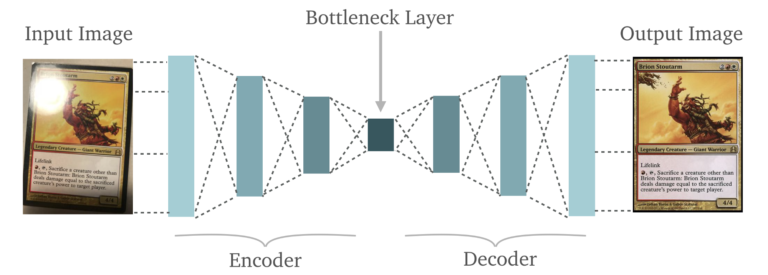
\includegraphics[width=0.8\linewidth]{images/feature-variation.png}
				\caption{Feature variation using autoencoders}
				\label{fig:feature-variation}
			\end{figure}
		
		\subsubsection{Other applications}

			Autoencoders are also used in other applications such as image compression, image generation, anomaly detection, image augmentation, and more.


	\subsection{Arhiteture of Autoencoders}
		Before we dive into the working of autoencoders, let us first introduce main parts that are used in autoencoders such as encoder, decoder, and bottleneck.

		\begin{figure}[h]
			\centering
			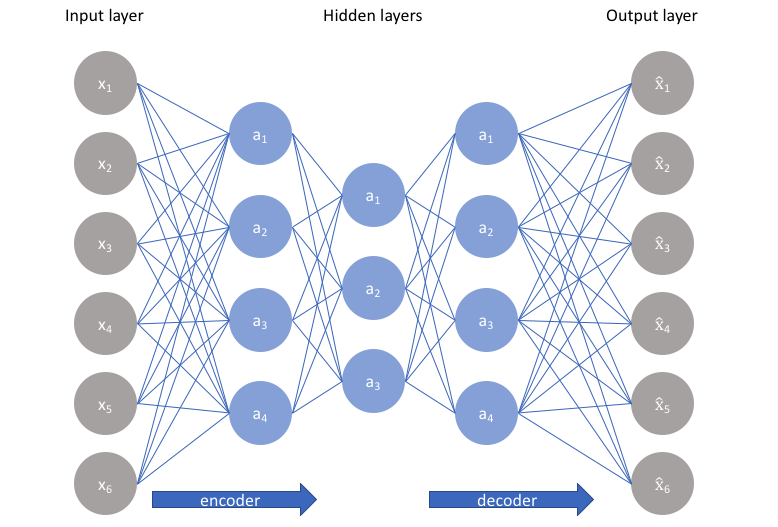
\includegraphics[width=0.5\linewidth]{images/encoder-decoder.png}
			\caption{Autoencoder architecture with encoder and decoder components}
			\label{fig:encoder-decoder}
		\end{figure}

		\subsubsection{Encoder}

			Encoder is a neural network that takes the input data and maps it to a lower dimensional representation, often referred to as the latent space. Mathematically, this can be represented as:

			\[ h = f_{\text{encoder}}(x) \]

			where \(x\) is the input data, \(h\) is the encoded representation, and \(f_{\text{encoder}}\) is the encoding function.
		
		\subsubsection{Bottleneck}


			Bottleneck represent middle layer of the network. It is a layer that has a smaller number of neurons compared to both encoder and decoder. This forces the network to reduce the information such that the noise is reduced, and they could only approximate the original data rather than copy it end-to-end.

			In essence bottleneck is a compression algorithm that compresses the input data into a lower dimensional representation. 

			It produces latent variables or so called latent representations introduced by Information Bottleneck method\footnote{introduced in 1999 by Naftali Tishby, Fernando C. Pereira, and William Bialek which hypothesis that it can extract vital information or representation by compressing the amount of information that can traverse through the network. This information is known as latent variables or latent representations. 
			}. 
			This random variables are extracted from the distribution and they give us abstract knowledge of the topology and the distribution of the data.

			The latent variables in above formula are denoted as \(h\)

		\subsubsection{Decoder}
			
			Decoder is a neural network that reconstructs the input data from the encoded representation. It aims to generate an output that is as close as possible to the original input. Mathematically, the decoding function is represented as:

			\[ x' = f_{\text{decoder}}(h) \]

			where \(x'\) is the reconstructed data, \(h\) is the encoded representation, and \(f_{\text{decoder}}\) is the decoding function.


	\subsection{Training Autoencoders}

		To train a basic autoencoder, the network is optimized to minimize the difference between the input data and the reconstructed output. This is often done by minimizing a loss function, such as mean squared error (MSE), between the input and output:

		The loss function \(\mathcal{L}\) is defined as follows:
		\begin{align}
			\mathcal{L}(x, x') &= \frac{1}{N} \sum_{i=1}^{N} \|x_i - x_i'\|^2 \\
			\text{where} \quad N &\text{ is the number of training samples,} \nonumber \\
			x_i &\text{ is the input data,} \nonumber \\
			x_i' &\text{ is the corresponding reconstructed output.} \nonumber
		\end{align}


	\subsection{Types of Autoencoders}

		The basic autoencoder architecture we discussed is known as the vanilla autoencoder. However, various modifications and extensions have been proposed, including:
		\begin{itemize}
			\item \textbf{Denoising Autoencoder:} Trained to remove noise from input data.
			\item \textbf{Sparse Autoencoder:} Introduces sparsity constraints in the encoded representation.
			\item \textbf{Variational Autoencoder (VAE):} Models probability distributions in the latent space.
		\end{itemize}


	\subsection{Sparse autoencoders}
		Sparse autoencoders offer us an alternative method for introducing an information bottleneck without requiring a reduction in the number of nodes at our hidden layers. Rather, we'll construct our loss function such that we penalize activations within a layer. For any given observation, we'll encourage our network to learn an encoding and decoding which only relies on activating a small number of neurons.

		\begin{figure}[H]
			\centering
			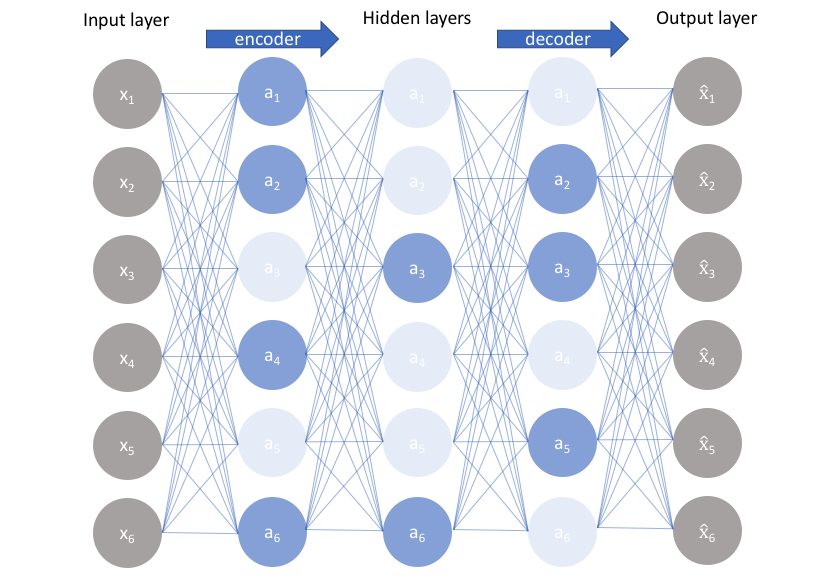
\includegraphics[width=0.8\linewidth]{images/sparse_autoencoder.png}
			\caption{Sparse autoencoder architecture}
			\label{fig:sparse-autoencoder}
		\end{figure}
			
		We should note that this is a different approach towards regularization, as we normally regularize the weights of a network, not the activations.

		There are two main ways by which we can impose this sparsity constraint; both involve measuring the hidden layer activations for each training batch and adding some term to the loss function in order to penalize excessive activations. These terms are:

		\subsubsection{Loss function}

		\textbf{L1 Regularization}: We can add a term to our loss function that penalizes the absolute value of the vector of activation \(a\) in layer \(h\) for observation \(i\) scaled by a tunning parameter \(\lambda\).

		\[ \mathcal{L}(x, x') = \frac{1}{N} \sum_{i=1}^{N} \|x_i - x_i'\|^2 + \lambda \sum_{j=1}^{m} |a_j^{(h)}| \]

		\textbf{KL-Divergence Regularization}: We can add a term to our loss function that penalizes the average activation. KL-Divergence measure of how one probability distribution differs from another. 

		Average activation of each neuron in the hidden layer \(h\) for a given training batch \(x'\) is defined as follows:
		\begin{align}
			\hat{\rho}_j &= \frac{1}{m} \sum_{i=1}^{m} a_j^{(h)}(x_i') \\
			\text{where} \quad m &\text{ represents the number of training samples (batch size),} \nonumber \\
			j &\text{ represents the } j\text{-th neuron in the hidden layer,} \nonumber \\
			a_j^{(h)}(x_i') &\text{ represents the activation of the } j\text{-th neuron in the hidden layer for the } i\text{-th training sample.} \nonumber
		\end{align}

		In essence, by constraining the average activation of a neuron over a collection of samples we're encouraging neurons to only fire for a subset of the observations.
		
		KL-Divergence is defined as follows:
		\begin{align}
			\text{KL}(\rho \| \hat{\rho}) &= \sum_{j=1}^{l^{(h)}} \rho \log\left(\frac{\rho}{\hat{\rho}_j}\right) + (1 - \rho) \log\left(\frac{1 - \rho}{1 - \hat{\rho}_j}\right) \\
			\text{where} \quad l^{(h)} &\text{ represents the number of neurons in the hidden layer,} \nonumber \\
			\rho &\text{ is the sparsity hyper parameter,} \nonumber \\
			\hat{\rho}_j &\text{ represents the average activation of the } j\text{-th neuron in the hidden layer.} \nonumber
		\end{align}
		

		So finally the loss function for KL-Divergence Regularization is defined as follows:
		\begin{align}
			\mathcal{L}(x, x') &= \frac{1}{N} \sum_{i=1}^{N} \|x_i - x_i'\|^2 + \lambda \sum_{j=1}^{m} \text{KL}(\hat{\rho} || \rho_j)
		\end{align}
		


	\subsection{Denoising}
		Autoencoders can be used to remove noise from data. This is done by training the network to reconstruct the original input from a input to which we artificialy added noise. 
		The goal is that network learns to extract the essential features from the input data and discard the noise. 

		\begin{figure}[H]
			\centering
			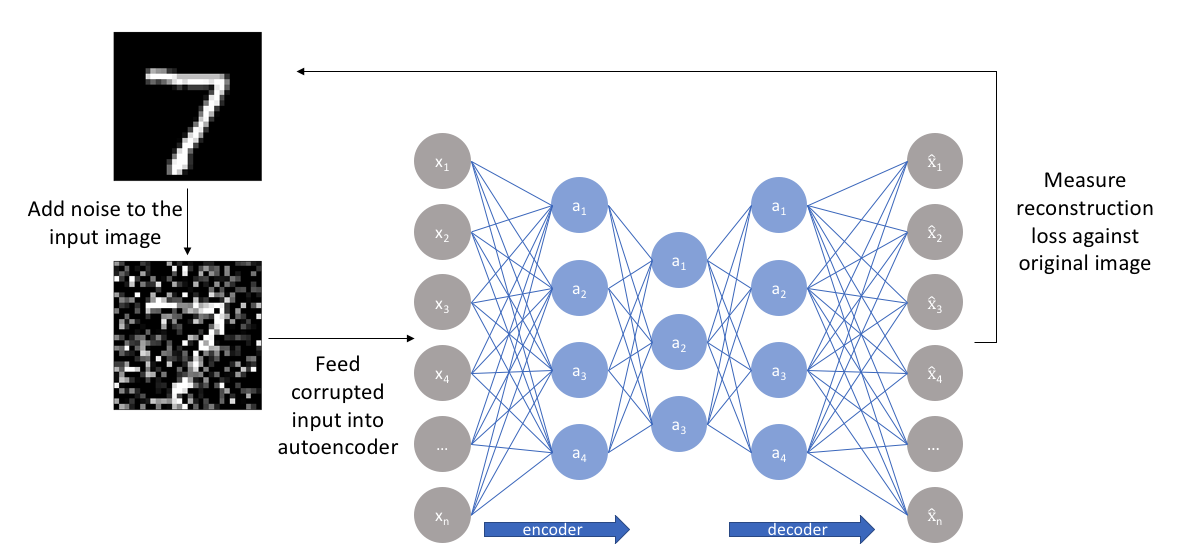
\includegraphics[width=0.8\linewidth]{images/denosing-autoencoder.png}
			\caption{Denoising autoencoder architecture}
			\label{fig:denoising}
		\end{figure}

		With this approach, our model isn't able to simply develop a mapping which memorizes the training data because our input and target output are no longer the same. Rather, the model learns a vector field for mapping the input data towards a lower-dimensional manifold. If this manifold accurately describes the natural data, we've effectively "canceled out" the added noise.

		\subsubsection{Corruption process}

			There are various ways to corrupt the input data. Some common approaches include:

			\begin{itemize}
				\item \textbf{Gaussian Noise:} Add random Gaussian noise to the input data.
				\item \textbf{Dropout:} Randomly set some input units to zero.
				\item \textbf{Masking Noise:} Randomly set some features of the input data to zero.
			\end{itemize}

		\subsubsection{Loss function}

			To train a denoising autoencoder, we define loss function as follows:

			\begin{align}
				\mathcal{L}_{\text{DAE}}(x, \tilde{x}, x') &= \frac{1}{N} \sum_{i=1}^{N} \|x_i - x_i'\|^2 \\
				\text{where} \quad N & : \text{Number of training samples,} \nonumber \\
				x_i & : \text{Clean data for the } i\text{-th training sample,} \nonumber \\
				\tilde{x}_i & : \text{Corrupted input for the } i\text{-th training sample,} \nonumber \\
				x_i' & : \text{Reconstructed output for the } i\text{-th training sample.} \nonumber
			\end{align}


			In comparing the loss functions of a denoising autoencoder and a vanilla autoencoder, a key distinction arises in the input provided to the encoder. In the denoising autoencoder, the encoder receives a corrupted input as \(\tilde{x}\). Then the decoder attempts to reconstruct the original input \(x\) from the encoded representation \(h\). 
			
			In contrast, the vanilla autoencoder receives the original input \(x\) and attempts to reconstruct the same input \(x\).

	\subsection{Variational Autoencoders (VAEs)}
			
		VAEs are a type of autoencoder that add probabilistic constraints to the latent space variables. This allows them to model probability distributions in the latent space.
		This models are widely used in applications such as image generation, image interpolation, and data augmentation.

		\begin{figure}[H]
			\centering
			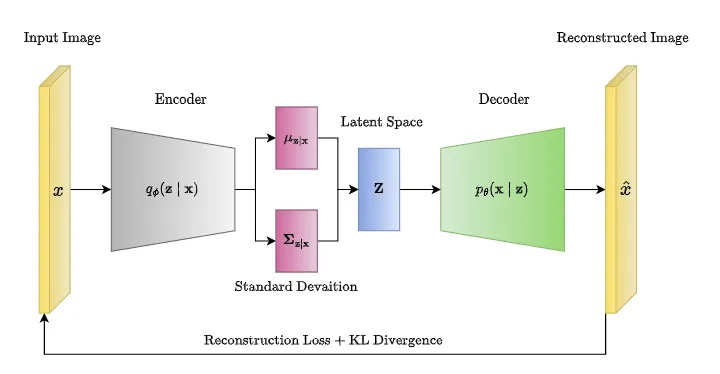
\includegraphics[width=0.8\linewidth]{images/vae.png}
			\caption{Variational autoencoder architecture}
			\label{fig:vae}
		\end{figure}

		\subsubsection{Latent space}

			In a vanilla autoencoder, encoder outputs a point in the latent space and decoder maps the point in the latent space to the reconstructed output. \newline 
			But in Variational Autoencoders, the encoder outputs mean vector \(\mu\) and a variance vector \(\sigma^2\) - so it outputs a probability distribution in the latent space and decoder maps the sample from the latent space to the reconstructed output. \newline
			Latent space is defined as follows:

			\[ h = z \sim \mathcal{N}(\mu, \sigma^2) \]

			where \(z\) is the latent vector, \(\mu\) is the mean vector, and \(\sigma^2\) is the variance vector.

			Instead of a single point in the latent space as in vanilla autoencoder, the VAE covers a certain “area” centered around the mean value with a size corresponding to the standard deviation. This gives the decoder a lot more to work with — a sample from anywhere in the area will be very similar to the original input
		
		\subsubsection{Latent space regularity}

			The regularity that is expected from the latent space in order to make the generative process possible requires:
			\begin{itemize}
			\item Continuity: Two close points in the latent space should not yield completely different contents once decoded.
			
			\item Completeness: For a chosen distribution, a point sampled from the latent space should result in "meaningful" content once decoded.
			\end{itemize}

			\begin{figure}[H]
				\centering
				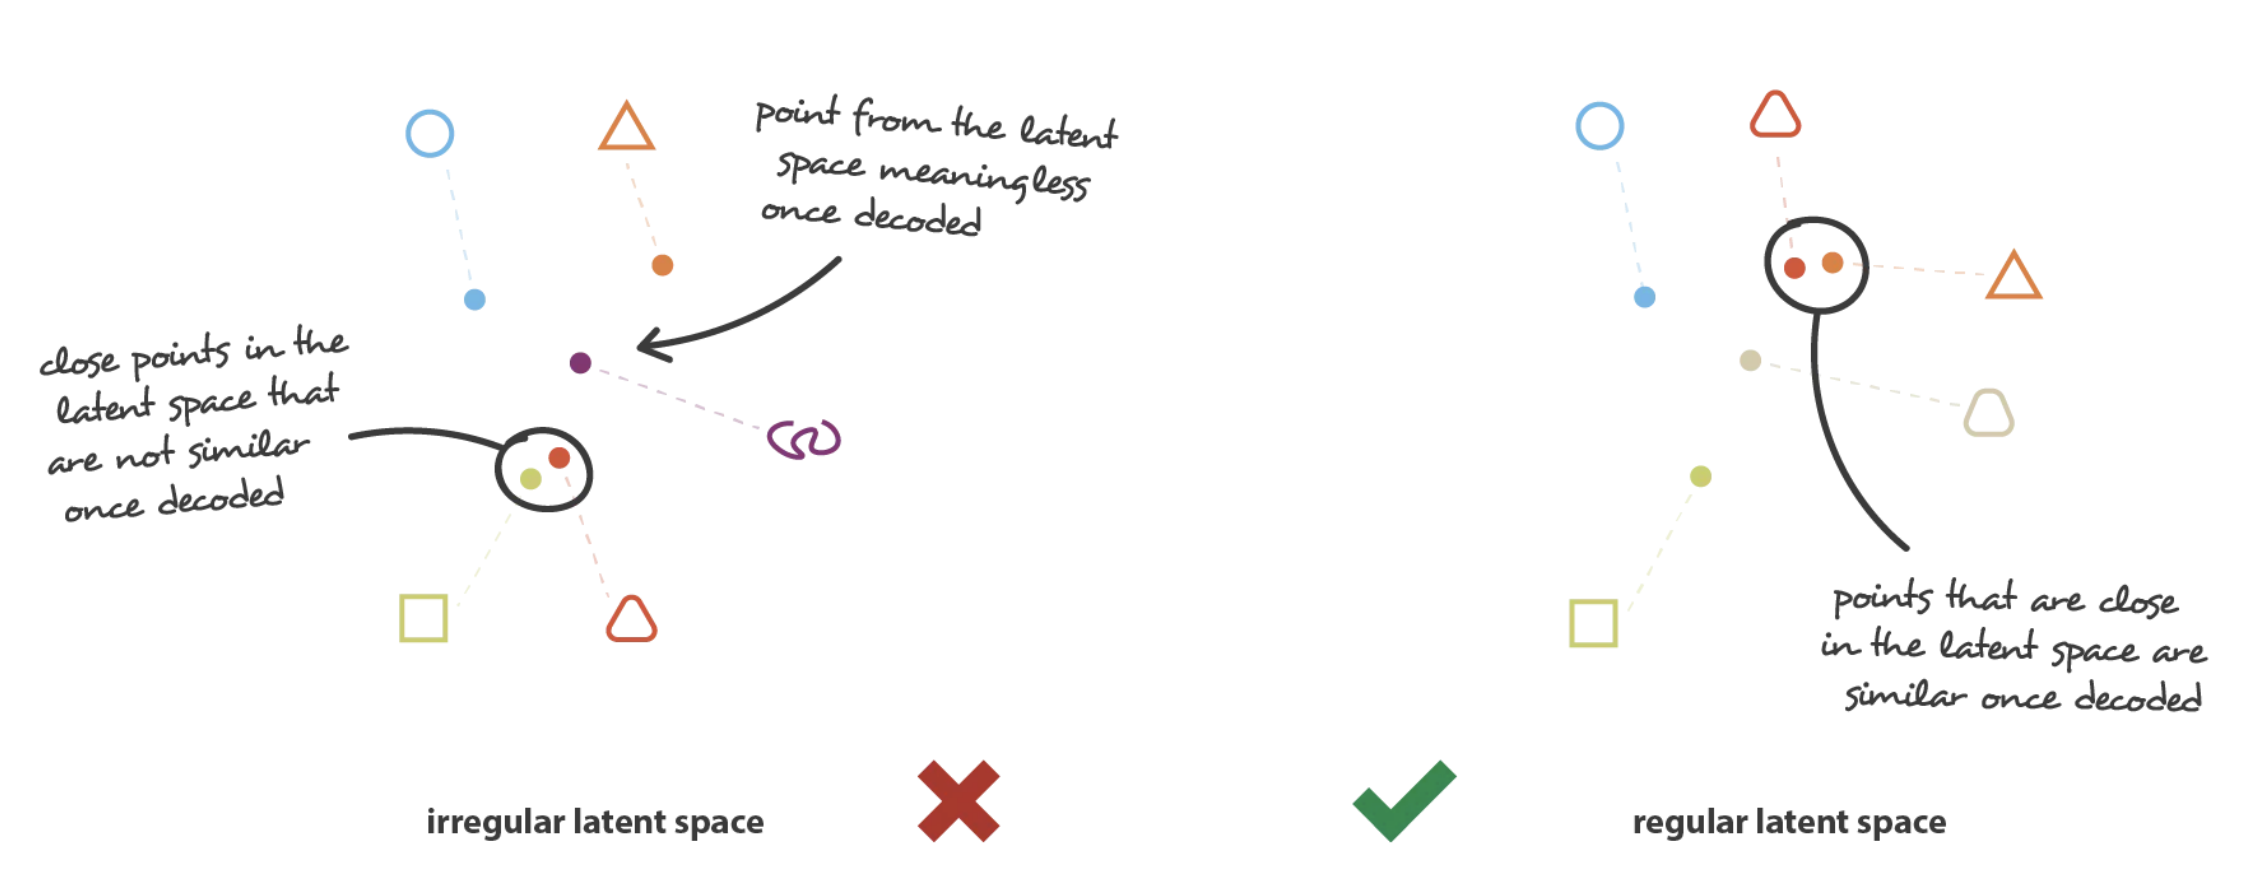
\includegraphics[width=0.8\linewidth]{images/var-irr-reg.png}
				\caption{Latent space regularity}
				\label{fig:var-irr-reg}
			\end{figure}

			In practice regularisation is done by enforcing distributions to be close to a standard normal distribution (centred and reduced). 
			So we can say that VAEs are regularized autoencoders whose encodings distribution is forced to be close to a standard normal distribution.
			\[
				Z \sim \mathcal{N}(0, 1)
			\]

			\begin{figure}[H]
				\centering
				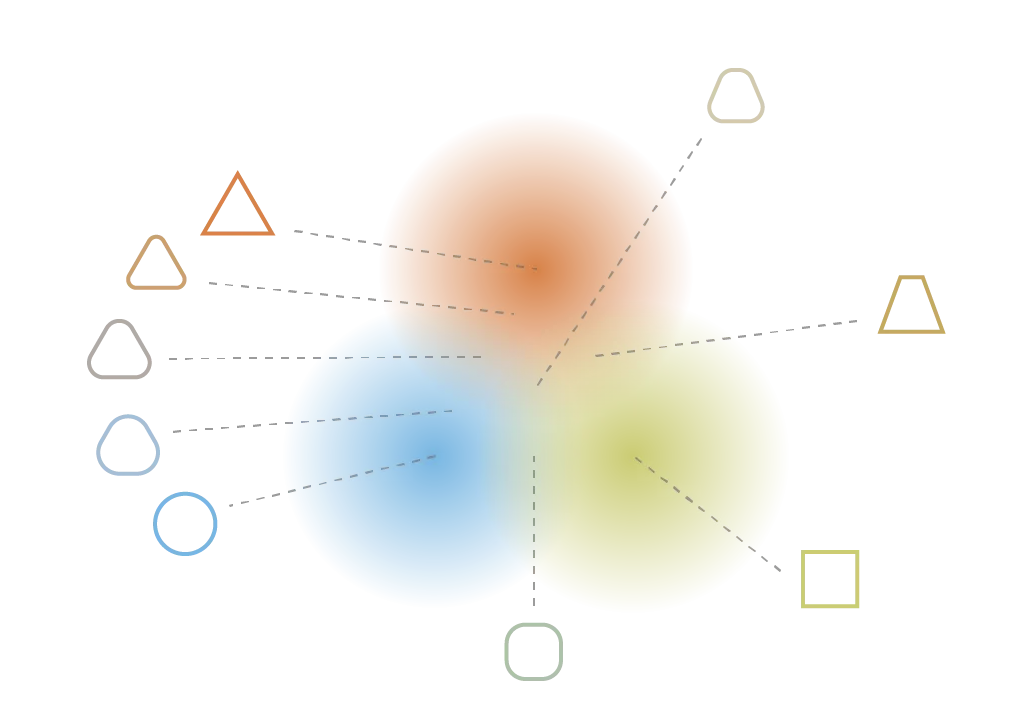
\includegraphics[width=0.8\linewidth]{images/vag-distribution.png}
				\caption{Latent space regularity distribution}
				\label{fig:vag-dist}
			\end{figure}


		\subsubsection{Reparameterization trick}

			To train a VAE, we need to sample from the latent space. However, we cannot directly sample from the latent space because it is a probability distribution. Instead, we use the reparameterization trick to sample from the latent space. The reparameterization trick is defined as follows:

			\[ z = \mu + \sigma \odot \epsilon \]

			where \(z\) is the latent vector, \(\mu\) is the mean vector, \(\sigma\) is the standard deviation vector, \(\epsilon\) is a random vector sampled from a standard normal distribution, and \(\odot\) represents element-wise multiplication.

		\subsubsection{Loss function}

			To train a VAE, we define the loss function as follows:

			\begin{align}
				\mathcal{L}_{\text{VAE}}(x, x') &= \frac{1}{N} \sum_{i=1}^{N} \|x_i - x_i'\|^2 + \text{KL}(q(z|x_i) || p(z))
			\end{align}

			where \(N\) is the number of training samples, \(x_i\) is the input data, \(x_i'\) is the reconstructed output, \(q(z|x_i)\) is the encoder distribution, \(p(z)\) is the prior distribution, and \(\text{KL}\) is the Kullback-Leibler divergence.

			The KL divergence term ensures that the learned distribution over the latent space is close to the prior distribution, which helps regularize the model and ensures that the latent space has a meaningful structure.


	\subsubsection{Applications}

			In comparison to traditional Autoencoders (AEs), VAEs introduce a probabilistic twist to the encoding-decoding process, enabling them to excel in generative tasks such as image generation, text generation, and data augmentation. 

			Major applications encompass:

			\begin{itemize}
				\item \textbf{Image Generation and Interpolation:} VAEs can generate new images that closely resemble the training dataset, facilitating tasks such as synthetic image creation and artistic design. Moreover, they are adept at interpolating between images, offering smooth transitions and understanding of semantic image features.
				
				\item \textbf{Data Augmentation:} In scenarios where data is scarce, VAEs can augment existing datasets by generating new data points, thereby enhancing the performance of machine learning models without the need for additional real data.
				
				\item \textbf{Generative Tasks in Various Domains:} Beyond image generation, VAEs are instrumental in text generation, speech synthesis, and music generation. They can also be applied to other domains such as molecular design and drug discovery.
				
				\item \textbf{Anomaly Detection:} By learning to reconstruct normal data, VAEs can identify anomalies or outliers in a dataset. This is particularly valuable in areas like fraud detection, where deviations from the norm are subtle yet critical.
			\end{itemize}

	\section{Generative adversarial networks}

		Generative adversarial networks, or GANs, revolutionized generative modeling. Introduced in 2014, GANs consist of a generator and a discriminator engaged in competitive learning. The generator creates realistic data samples from random noise, refining its output through training iterations. Simultaneously, the discriminator learns to differentiate between real and generated samples. This adversarial interplay results in the generation of high-quality, realistic data. GANs are widely applied in tasks such as image synthesis, style transfer, and data augmentation.

		\begin{figure}[H]
			\centering
			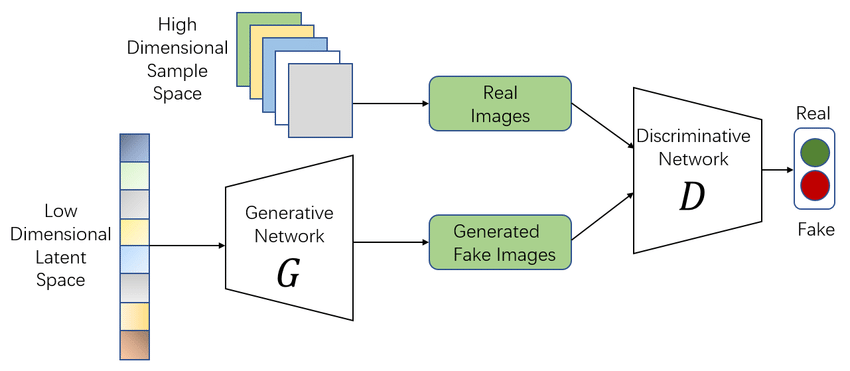
\includegraphics[width=0.8\linewidth]{images/gan-arhitecture.png}
			\caption{Generative adversarial network representation}
			\label{fig:gan}
		\end{figure}

		\subsection{Generator}

			The generator takes a random noise vector as input and generates a sample from the data distribution. The generator is trained to fool the discriminator into classifying the generated sample as real.

		\subsection{Discriminator}

			The discriminator takes a sample from the data distribution or a generated sample as input and classifies it as real or fake. The discriminator is trained to correctly classify the real samples as real and the generated samples as fake.

		\subsection{Training}

			The generator and discriminator are trained simultaneously in a competitive process. The generator is trained to fool the discriminator into classifying the generated sample as real. The discriminator is trained to correctly classify the real samples as real and the generated samples as fake. This adversarial interplay results in the generation of high-quality, realistic data.

			\begin{figure}[H]
				\centering
				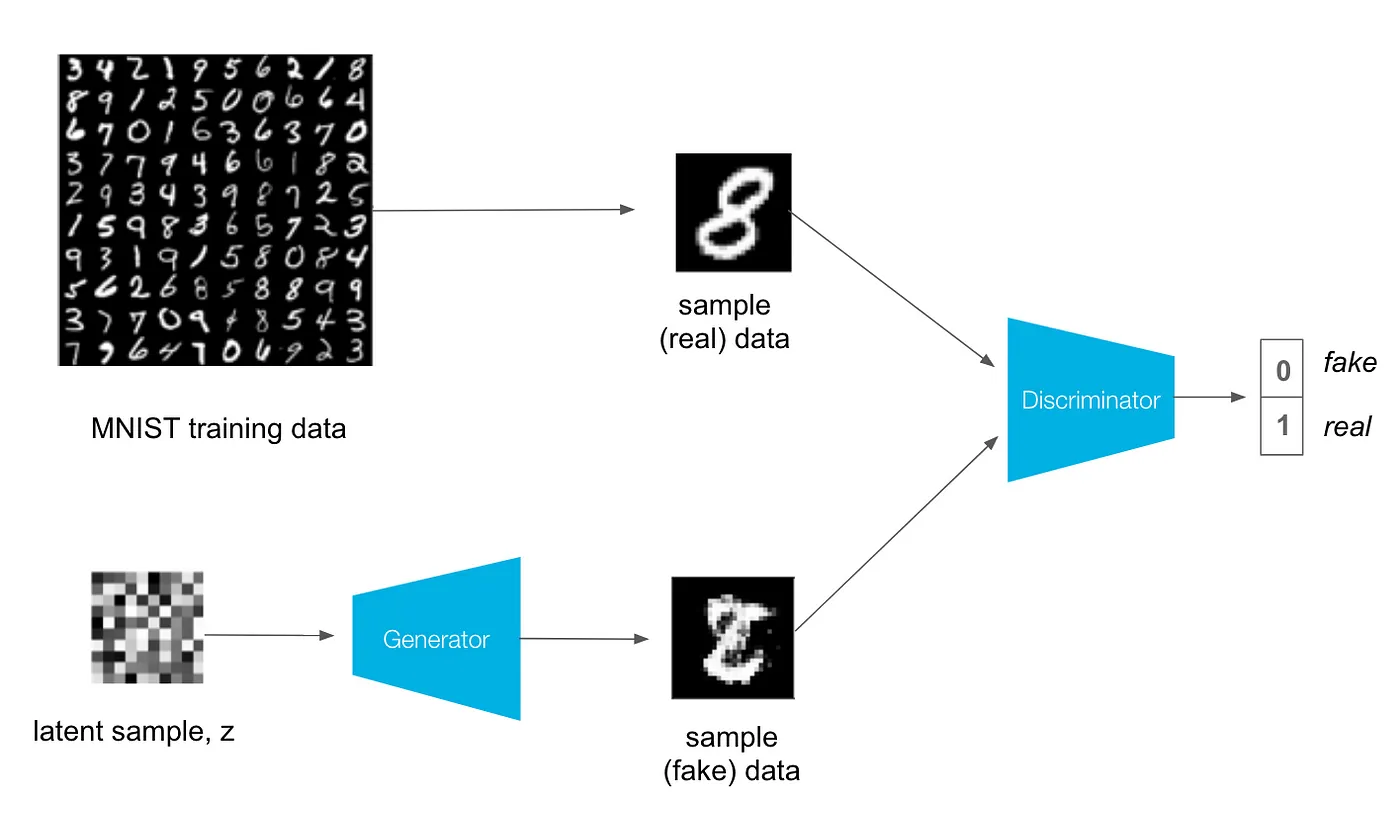
\includegraphics[width=0.8\linewidth]{images/gan-training.png}
				\caption{GAN training process}
				\label{fig:gan-training}
			\end{figure}

		\subsection{Loss function}

			The loss function for the generator is defined as follows:

			\begin{align}
				\mathcal{L}_{\text{generator}}(z) &= \log(1 - D(G(z)))
			\end{align}

			where \(z\) is the random noise vector, \(G\) is the generator, \(D\) is the discriminator, and \(\mathcal{L}_{\text{generator}}\) is the loss function for the generator.

			The loss function for the discriminator is defined as follows:

			\begin{align}
				\mathcal{L}_{\text{discriminator}}(x, z) &= -\log(D(x)) - \log(1 - D(G(z)))
			\end{align}

			where \(x\) is the input data, \(z\) is the random noise vector, \(G\) is the generator, \(D\) is the discriminator, and \(\mathcal{L}_{\text{discriminator}}\) is the loss function for the discriminator.

		\subsection{Applications}

			GANs are widely applied in tasks such as image synthesis, style transfer, and data augmentation.

			\subsubsection{Image Synthesis}

				GANs can generate realistic images that closely resemble the training dataset. This is particularly valuable in scenarios where data is scarce, such as in medical imaging. GANs can also be used to generate images from text descriptions, enabling applications such as image captioning.

			\subsubsection{Style Transfer}

				GANs can transfer the style of one image to another, enabling applications such as image colorization and image-to-image translation. This is achieved by training the generator to translate an image from one domain to another, while the discriminator learns to distinguish between real and generated images.

			\subsubsection{Data Augmentation}

				In scenarios where data is scarce, GANs can augment existing datasets by generating new data points, thereby enhancing the performance of machine learning models without the need for additional real data.

	\section{Diffusion Models}

		Inspired by physical processes like molecular diffusion, diffusion models simulate the gradual generation of data. They apply a series of transformations iteratively to a base distribution. This iterative process progressively refines the base distribution until it converges to the desired data distribution.

		So this models operate by simulating a diffusion process, which transforms data into a Gaussian random noise through a predefined number of steps and the essence of diffusion models lies in learning the reverse process—starting from noise and gradually reconstructing the data.

		Diffusion models have emerged as a powerful class of generative models, achieving state-of-the-art results in generating high-fidelity images, audio, and text.

		\begin{figure}[H]
			\centering
			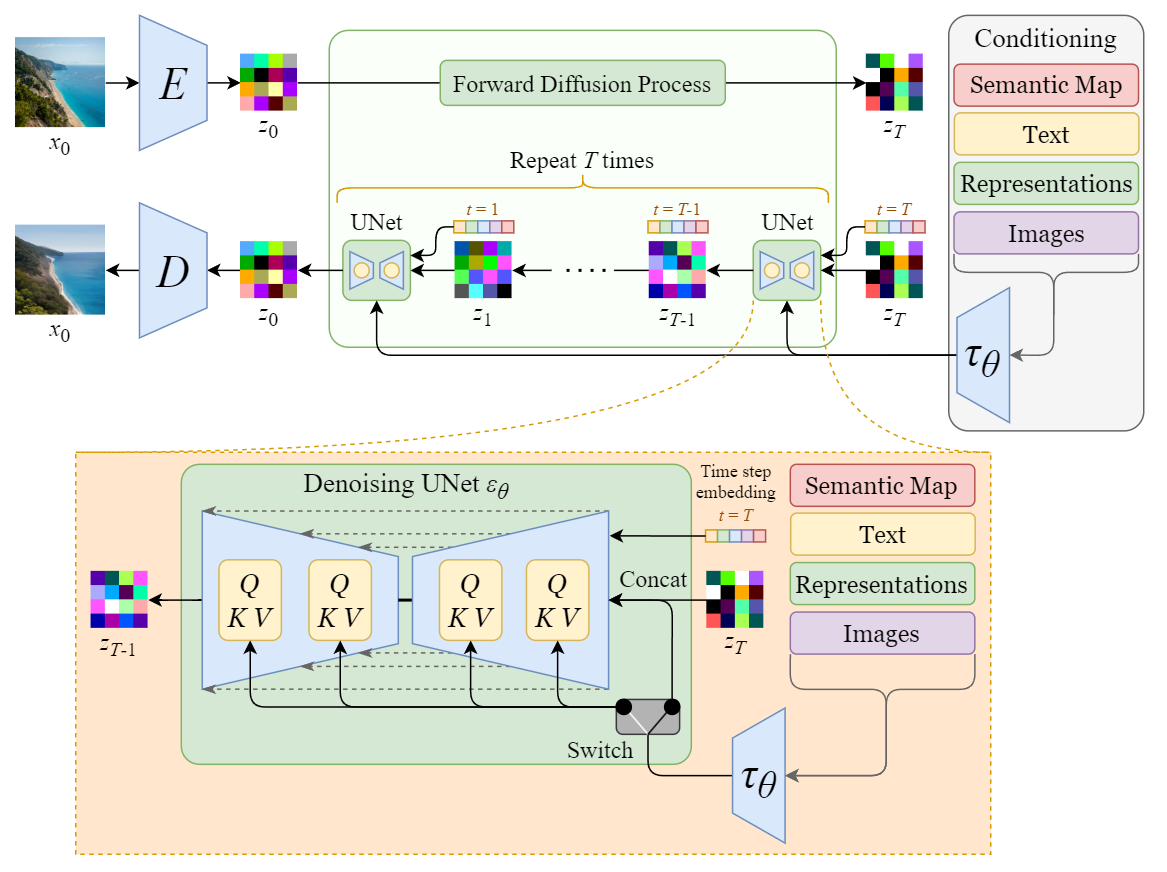
\includegraphics[width=0.8\linewidth]{images/diffusion-model.png}
			\caption{Diffusion model architecture}
			\label{fig:diffusion-model}
		\end{figure}

		\subsection{How Diffusion Models Work}
			The workflow of diffusion models can be divided into two phases: the forward diffusion phase and the reverse diffusion phase. The forward phase incrementally adds Gaussian noise to the data across a series of steps, until the data is completely indistinguishable from random noise. Mathematically, this process can be expressed as:
			\begin{equation}
			x_{t} = \sqrt{\alpha_t} x_{t-1} + \sqrt{1 - \alpha_t} \epsilon, \quad \epsilon \sim \mathcal{N}(0, \mathbf{I}),
			\end{equation}
			where $x_t$ represents the data at step $t$, $\alpha_t$ is a variance schedule, and $\epsilon$ is sampled from a standard Gaussian distribution.

			The reverse phase, on the other hand, involves a neural network model learning to estimate the clean data from the noisy data, effectively reversing the diffusion process. This is achieved by training the model to predict the noise that was added at each step, gradually denoising the input until it recovers the original data. The reverse process can be expressed as:
			\begin{equation}
			x_{t-1} = \frac{x_t - \sqrt{1 - \alpha_t} \epsilon}{\sqrt{\alpha_t}},
			\end{equation}
			where $x_{t-1}$ represents the data at step $t-1$, $x_t$ is the noisy data at step $t$, $\alpha_t$ is a variance schedule, and $\epsilon$ is the noise added at step $t$. The goal of the reverse process is to estimate the clean data from the noisy data, effectively denoising the input.

		\subsection{Mathematical Formulation of the Loss Function}
			The training of diffusion models is guided by a loss function that encourages the model to accurately reverse the diffusion process. A commonly used loss is the variational lower bound, which can be formulated as:
			\begin{equation}
				\mathcal{L}_{\text{{total}}} = \mathbb{E}_{x_0,\epsilon}\left[\log p_\theta(x_0|x_T) + \sum_{t=1}^{T}\log p_\theta(x_{t-1}|x_t)\right],
			\end{equation} 
			represents the total loss calculated across all diffusion steps.
			where $p_\theta$ denotes the model's distribution parameterized by $\theta$, and $T$ is the total number of diffusion steps. This loss function combines the log-likelihood of the original data given the final noisy data and the log-likelihood of each reverse step, effectively measuring the model's ability to reconstruct the original data from noise.

			Another loss function that is used is the Kullback-Leibler divergence, which can be formulated as:

			\begin{equation}
				\mathcal{L}_{\text{{total}}} = \mathbb{E}_{x_0,\epsilon}\left[\log p_\theta(x_0|x_T) + \sum_{t=1}^{T}KL(q(x_{t-1}|x_t, x_0)||p_\theta(x_{t-1}|x_t))\right],
			\end{equation}
			represents the total loss calculated across all diffusion steps.
			where $p_\theta$ denotes the model's distribution parameterized by $\theta$, and $T$ is the total number of diffusion steps. This loss function combines the log-likelihood of the original data given the final noisy data and the Kullback-Leibler divergence of each reverse step, effectively measuring the model's ability to reconstruct the original data from noise. \\

			Both equations aim to minimize the difference between the original data and the data generated by reversing the diffusion process, thereby training the model to accurately reconstruct data from noise. The first equation focuses on maximizing the likelihood of each reverse step directly, while the second equation also incorporates the KL divergence to ensure the model's distribution closely matches the true generative process.
	
		
		\subsection{Breakthroughs and Training Process}

			Diffusion models have seen significant breakthroughs in recent years, including improvements in sampling efficiency, model architecture, and training techniques. These advancements have enabled diffusion models to generate highly realistic and diverse outputs across various domains.
			
			The training process of diffusion models involves iteratively applying the forward diffusion to the training data, and then training the model to predict the reverse diffusion steps. This requires careful balancing of the noise levels and ensuring the model can effectively learn the data distribution. Advanced techniques, such as learning rate schedules and architecture designs, have been developed to optimize this process.

			So the diffusion model is trained by applying a series of transformations iteratively to a base distribution. This iterative process progressively refines the base distribution until it converges to the desired data distribution, this we can see in the figure \ref{fig:diffusion-model-training}.

			\begin{figure}[H]
				\centering
				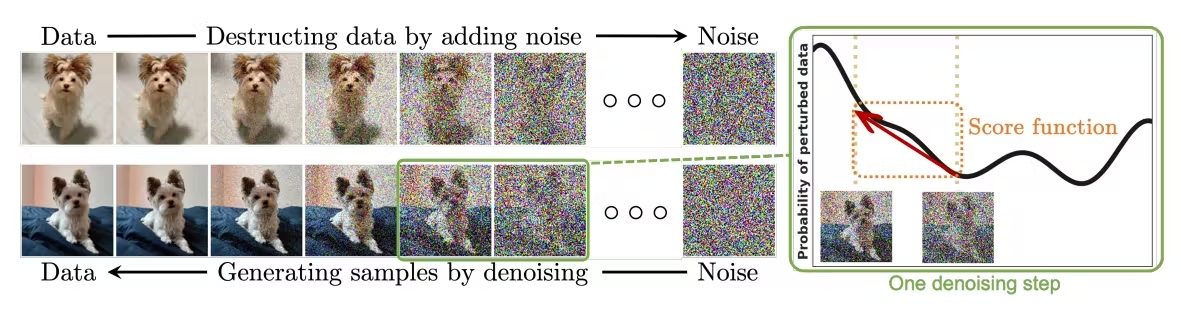
\includegraphics[width=0.8\linewidth]{images/diffusion-training.jpg}
				\caption{Diffusion model training}
				\label{fig:diffusion-model-training}
			\end{figure}

		\subsection{Applications and Future Prospects}

			The application spectrum of diffusion models is vast and continually expanding, covering areas from photorealistic image generation to the synthesis of human-like speech. The fidelity and versatility of the outputs have opened new frontiers in content creation, medical imaging, and beyond. Looking ahead, the exploration of diffusion models in unsupervised learning, domain adaptation, and their integration with other AI modalities heralds a promising trajectory for future research and application.

		
		\section{Conclusion}

			Throughout this report, we have introduced and examined three prominent generative models in machine learning: \textbf{Autoencoders}, \textbf{Generative Adversarial Networks (GANs)}, and \textbf{Diffusion Models}.

			\begin{figure}[H]
				\centering
				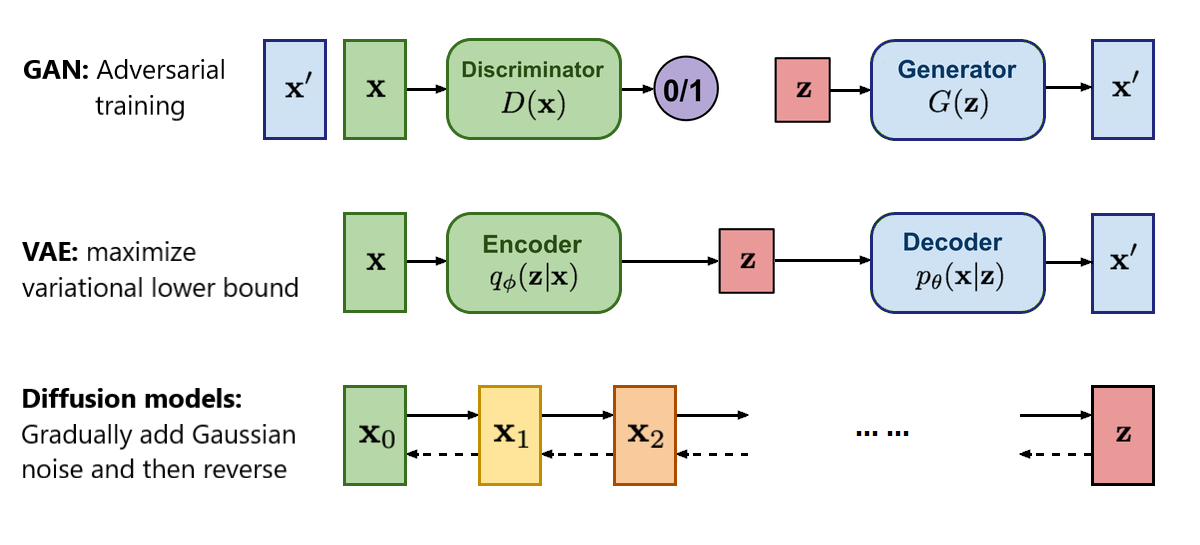
\includegraphics[width=0.8\linewidth]{images/gan-vae-diffusin.png}
				\caption{Conceptual summary of autoencoders, GANs, and diffusion models}
				\label{fig:summary}
			\end{figure}

			Autoencoders are notable for their ability in data compression and reconstruction, making them a potent tool for dimensionality reduction, denoising, and feature extraction. Their architecture, comprising an encoder and a decoder, enables efficient data representation, critical for tasks that demand data compression with minimal information loss.

			Generative Adversarial Networks (GANs) have transformed synthetic data generation. Utilizing a competitive mechanism between a generator and a discriminator, GANs can create highly realistic images, texts, and other data forms. This capability not only improves synthetic data quality but also opens new avenues in art creation, photo editing, and game development, where realistic content generation is crucial.

			Diffusion Models, the forefront of generative model technology, are inspired by the natural diffusion process. These models convert data into a noise-like distribution and then learn to reverse this transformation to generate data. They excel in producing realistic and varied outputs, establishing new benchmarks for realism and detail in generated content. Demonstrating superior performance in text-to-image synthesis, audio generation, and beyond, diffusion models highlight their versatility and promise for future exploration and application.

			In conclusion, autoencoders, GANs, and diffusion models each offer distinctive approaches to understanding and generating complex data. Autoencoders are adept at learning efficient data representations, GANs at generating realistic synthetic data, and diffusion models at creating high-quality content through a novel reverse diffusion process. Collectively, these technologies exemplify the swift advancements in machine learning, paving the way towards a future where generating and interpreting complex data is achieved with unparalleled precision and creativity.



		\newpage
		\section{References}
		\begin{enumerate}
			\item K. Preechakul, N. Chatthee, S. Wizadwongsa, and S. Suwajanakorn, "Diffusion Autoencoders: Toward a Meaningful and Decodable Representation," \textit{Vidyasirimedhi Institute of Science and Technology}, Rayong, Thailand, 2022. [Online]. Available: \url{https://diff-ae.github.io/}

			\item J. Jordan, "Introduction to autoencoders", \textit{Jeremy Jordan's 
			Blog}, [Online]. Available: \url{https://www.jeremyjordan.me/autoencoders/}

			\item H. Bandyopadhyay, "Autoencoders in Deep Learning: Tutorial and Use Cases [2023]", \textit{V7 Labs Blog}, [Online]. Available: \url{https://www.v7labs.com/blog/autoencoders-guide}

			\item "How to Work with Autoencoders [Case Study Guide]", \textit{Neptune.ai Blog}, [Online]. Available: \url{https://neptune.ai/blog/autoencoders-case-study-guide}
			
			\item "Autoencoders Tutorial", \textit{Edureka Blog}, [Online]. Available: \url{https://www.edureka.co/blog/autoencoders-tutorial/}
			
			\item R. Shende, ``Autoencoders, Variational Autoencoders (VAE), and \(\beta\)-VAE'', \textit{Medium Blog}, [Online]. Available: \url{https://medium.com/@rushikesh.shende/autoencoders-variational-autoencoders-vae-and-\%CE\%B2-vae-ceba9998773d}
			\item "Variational Autoencoder in TensorFlow", \textit{LearnOpenCV Blog}, [Online]. Available: \url{https://learnopencv.com/variational-autoencoder-in-tensorflow/}
			
			\item K. Preechakul, N. Chatthee, S. Wizadwongsa, and S. Suwajanakorn, "Diffusion Autoencoders: Toward a Meaningful and Decodable Representation," in \textit{CVPR}, 2022. [Online]. Available: \url{https://openaccess.thecvf.com/content/CVPR2022/papers/Preechakul_Diffusion_Autoencoders_Toward_a_Meaningful_and_Decodable_Representation_CVPR_2022_paper.pdf}
			
			\item N. Siddiqui, "Comparative Study f Generative Models for Text-to-Image o-Image Generation", \textit{University of Windsor}, [Online]. Available: \url{https://scholar.uwindsor.ca/cgi/viewcontent.cgi?article=9960&context=etd}
			
			\item R. O'Connor, "How DALL-E 2 Actually Works", \textit{AssemblyAI Blog}, [Online]. Available: \url{https://www.assemblyai.com/blog/how-dall-e-2-actually-works/}
			
			\item R. O'Connor, "Diffusion Models for Machine Learning: Introduction", \textit{AssemblyAI Blog}, [Online]. Available: \url{https://www.assemblyai.com/blog/diffusion-models-for-machine-learning-introduction/}
		\end{enumerate}
		
		
		
		
		
	
\end{document}
